\documentclass[a4paper,10pt,twocolumn]{article}

% To include images
\usepackage{graphicx}

% Change the margins of the document
\usepackage[top=1cm,bottom=2cm,left=1cm,right=1cm]{geometry}

% No indentation but a wider space between the paragraphs
\setlength{\parindent}{0cm}
\setlength{\parskip}{2mm}

% Add a rule between the two columns and enlarge the space
\setlength{\columnseprule}{.5pt}
\setlength{\columnsep}{1cm}

% French language
\usepackage[francais]{babel}
\usepackage[utf8]{inputenc}

% Math extensions
\usepackage{amsfonts}
\usepackage{amstext}
\usepackage{amsmath}
\usepackage{mathbbol}

% Customize theorems
\usepackage{theorem}
\theoremstyle{break}

% Some useful shortcuts
\newcommand{\code}[1]{\mathcal{#1}}
\newcommand{\C}{\code{C}}
\newcommand{\syn}[1]{\mathop{\rm{syn}}(#1)}
\newcommand{\dimc}[1]{\mathop{\rm{dim}}(#1)}
\newcommand{\F}{\mathbb{F}}
\newcommand{\Poly}{\mathbb{P}}
\newcommand{\FF}{\F_2}
\newcommand{\FFn}[1]{\FF^{#1}}
\newcommand{\Zn}[1]{\mathbb{Z}_{#1}}
\newcommand{\Zp}{\Zn{p}}
\newcommand{\dg}[1]{\mathrm{d}^\circ(#1)}
\newcommand{\cy}[1]{{<}#1{>}}

% Definition of new environments
\newtheorem{mydef}{Définition}
\newtheorem{myprop}{Proposition}
\newtheorem{myth}{Théorème}
\newtheorem{mylemma}{Lemme}
\newtheorem{mycor}{Corolaire}

\newenvironment{note}[1]
{\textbf{#1}:}
{}

\newenvironment{mydem}
{\begin{note}{Démonstration}}
{\end{note}}

\newenvironment{myproof}
{\begin{note}{Preuve}}
{\end{note}}

\newenvironment{remarque}
{\begin{note}{Remarque}}
{\end{note}}

\newenvironment{proprietes}
{\begin{note}{Propriétés}}
{\end{note}}

\newenvironment{exemple}
{\begin{note}{Exemple}}
{\end{note}}

% Metadata
\title{Codes correcteurs d'erreur}
\author{Nicolas MASSE \\ \texttt{nicolas27.masse@laposte.net}}

\begin{document}

\maketitle

\begin{abstract}
 Ce document rassemble mes notes et mes travaux personnels relatifs aux cours de codes correcteurs d'erreur de M.~\textsc{Otmani} à l'ENSICAEN.
\end{abstract}

\tableofcontents
\clearpage

\section{Contexte}
\textbf{Objectif:} Convoyer à partir de la source vers le récepteur à travers un médium physique (le canal) de l'information de manière fiable.

\includegraphics[width=\linewidth]{general1}

\textbf{2 situations:}
\begin{enumerate}
 \item information transmise d'un point à un autre dans l'espace
 \item information transmise d'un point à un autre dans le temps
\end{enumerate}

\section{Décomposition d'un système de communication}
Shannon a montré en 1948 que la communication point à point peut être décomposée de la manière suivante.

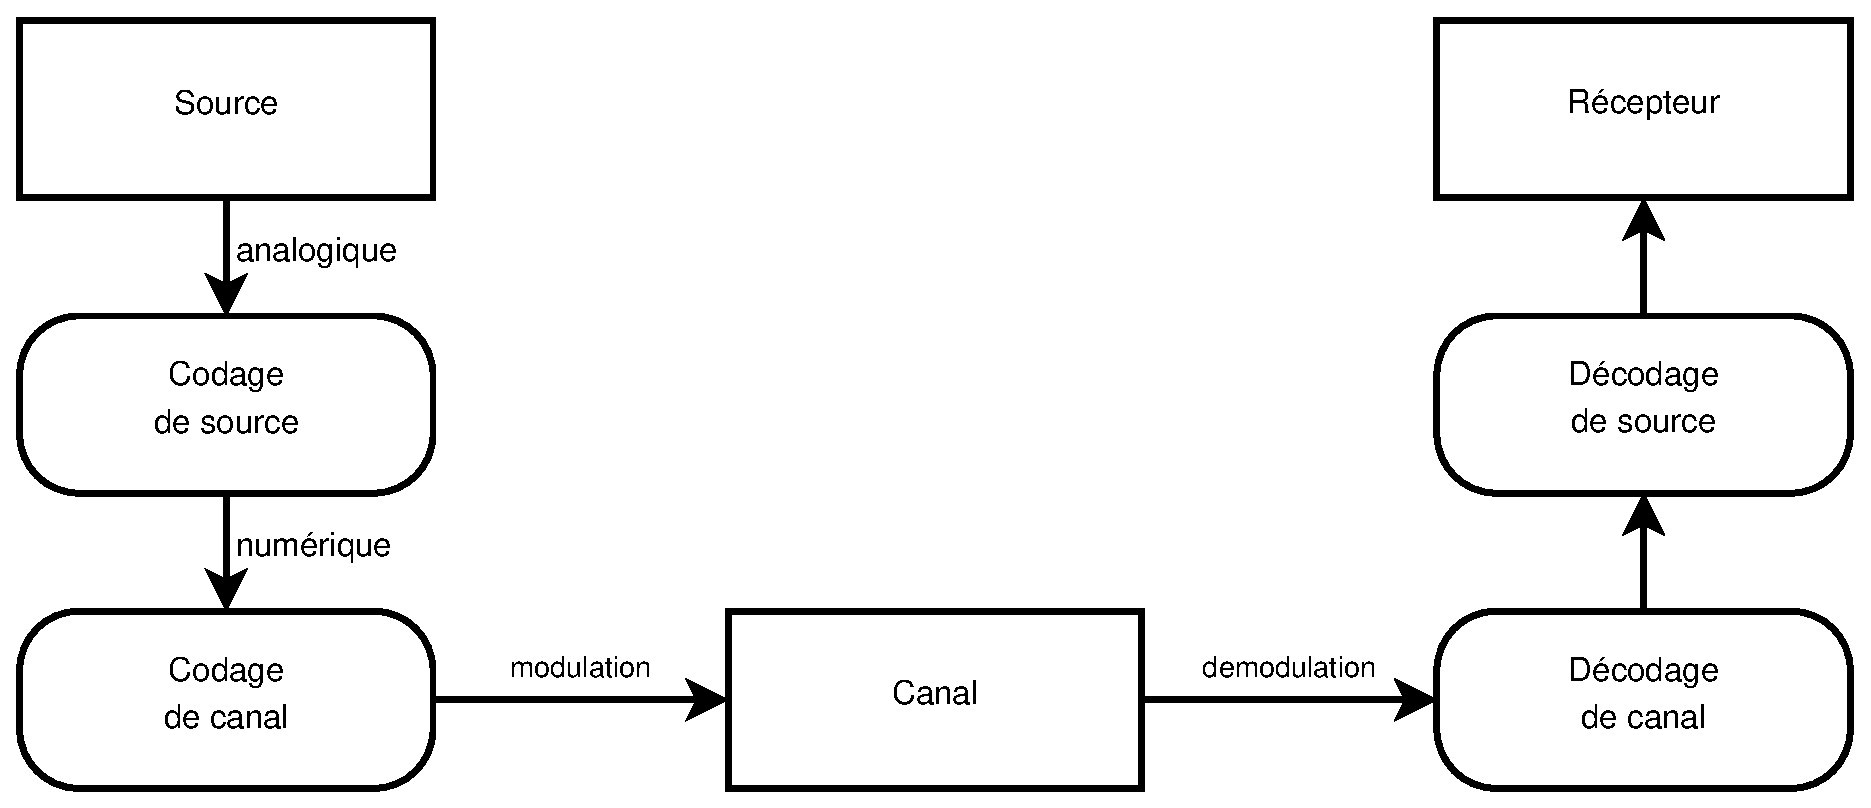
\includegraphics[width=\linewidth]{general2}

\subsection{Codage de source}
Il comprend:
\begin{itemize}
 \item échantillonnage
 \item quantification
 \item compression
\end{itemize}
Ce mécanisme a pour but de représenter sous forme linéaire le signal de manière efficace et fidèle.

\subsection{Codage de canal}
Ajouter de la redondance afin de lutter contre les perturbations dues au canal. 
Le codage de canal prend en entrée $k$ symboles binaires et donne $n$ symboles binaires, avec $n > k$

\section{Théorie des codes}
Le but de la théorie des codes est de concevoir des systèmes d'encodage et de décodage efficaces:
\begin{itemize}
 \item nombre d'opérations acceptable
 \item capacité de détection
 \item capacité de correction
\end{itemize}

\section{Quelques codes}
\subsection{Forward error correction (FEC)}
On ajoute de la redondance pour corriger, il n'y a pas de retransmission. ($ \ne $ checksum)

\subsection{Automatic Repeat-request (ARQ)}
Lorsqu'une erreur est détectée, on demande la retransmission de l'information erronée.
\begin{itemize}
 \item Stop and Wait
 \item Go back N
 \item Selective Repeat ARQ
\end{itemize}

\subsection{Code de Hamming}
On considère des messages de 4 bits et on ajoute 3 bits de redondance. C'est-à-dire qu'on émet $m_1 m_2 m_3 m_4 p_1 p_2 p_3$, avec:
\begin{eqnarray*}
p_1 & = & m_1 \oplus m_3 \oplus m_3 \\
p_2 & = & m_1 \oplus m_2 \oplus m_4 \\
p_3 & = & m_1 \oplus m_3 \oplus m_4 
\end{eqnarray*}

Le décodeur reçoit: $m_1' m_2' m_3' m_4' p_1' p_2' p_3'$ et calcule:
$$ \left(\begin{array}{c}
 S_1\\
 S_2\\
 S_3
\end{array}\right) $$
avec: 
$$\left\lbrace
\begin{array}{c}
S_1 = p_1' \oplus m_1' \oplus m_3' \oplus m_3' \\
S_2 = p_2' \oplus m_1' \oplus m_2' \oplus m_4' \\
S_3 = p_3' \oplus m_1' \oplus m_3' \oplus m_4' 
\end{array}\right.$$

Si la transmission est sans erreur, alors:
$$ \left(\begin{array}{c}
 S_1\\
 S_2\\
 S_3
\end{array}\right) =
 \left(\begin{array}{c}
 0\\
 0\\
 0
\end{array}\right) $$

S'il y a une erreur:

\begin{itemize}
 \item Si $m_1$ est faux
 $$ \left(\begin{array}{c}
 S_1\\
 S_2\\
 S_3
\end{array}\right) =
 \left(\begin{array}{c}
 1\\
 1\\
 1
\end{array}\right) $$
 \item Si $m_2$ est faux
 $$ \left(\begin{array}{c}
 S_1\\
 S_2\\
 S_3
\end{array}\right) =
 \left(\begin{array}{c}
 1\\
 1\\
 0
\end{array}\right) $$
 \item Si $m_3$ est faux
 $$ \left(\begin{array}{c}
 S_1\\
 S_2\\
 S_3
\end{array}\right) =
 \left(\begin{array}{c}
 1\\
 0\\
 1
\end{array}\right) $$
 \item Si $m_4$ est faux
 $$ \left(\begin{array}{c}
 S_1\\
 S_2\\
 S_3
\end{array}\right) =
 \left(\begin{array}{c}
 0\\
 1\\
 1
\end{array}\right) $$
 \item Si $p_1$ est faux
 $$ \left(\begin{array}{c}
 S_1\\
 S_2\\
 S_3
\end{array}\right) =
 \left(\begin{array}{c}
 1\\
 0\\
 0
\end{array}\right) $$
 \item Si $p_2$ est faux
 $$ \left(\begin{array}{c}
 S_1\\
 S_2\\
 S_3
\end{array}\right) =
 \left(\begin{array}{c}
 0\\
 1\\
 0
\end{array}\right) $$
 \item Si $p_3$ est faux
 $$ \left(\begin{array}{c}
 S_1\\
 S_2\\
 S_3
\end{array}\right) =
 \left(\begin{array}{c}
 0\\
 0\\
 1
\end{array}\right) $$

\end{itemize}

\textbf{Conclusion:} On peux corriger une erreur et en détecter deux.

\section{Encodeur-décodeur de canal}
L'encodeur traite les bits du message d'info par bloc de $k$ bits pour générer $n$ symboles binaires.

\begin{mydef}
 Le rendement d'un code est $ R = \frac{k}{n} $.
\end{mydef}

Après encodage, chaque symbole $C_i$ \flqq porte\frqq $R$ bits d'information. 
À l'inverse, pour retrouver un bit d'information, il faut $\frac{1}{R}$ bits.
Plus le rendement est faible, plus le nombre de bits pour reconstituer le message est important.

L'encodage doit être réversible, c'est-à-dire que:
$$ f: \{\text{Ensemble des messages d'information}\} \rightarrow \FFn{2} $$
et que $f$ est injective.

Le décodeur doit retrouver $\hat{C_1}, \ldots, \hat{C_n}$ qui est une estimation de $C_1, \ldots, C_n$ à partir de:
\begin{itemize}
 \item $C'_1, \ldots, C'_n$
 \item modèle de canal choisi
 \item encodeur de canal choisi
\end{itemize}

En sortie, on retrouve $(\hat{m_1}$, ..., $\hat{m_n})$ en inversant la fonction d'encodage $f$.

Quand $(\hat{m_1}, \ldots, \hat{m_k}) \ne (m_1, \ldots, m_k)$, le décodeur a commis une erreur.

En résumé, un codeur efficace a:
\begin{itemize}
 \item un rendement proche de 1
 \item une complexité faible
\end{itemize}

et un décodeur efficace a:
\begin{itemize}
 \item la complexité la plus faible possible
 \item la probabilité d'erreur la plus faible possible
\end{itemize}

\section{Modèle de canal}
\begin{mydef}
 Un canal est la donnée,
 \begin{itemize}
  \item $X$, alphabet d'entrée;
  \item $Y$, alphabet de sortie;
  \item pour tout $x \in X$, $y \in Y$, la probabilité conditionnelle $P(x/y)$, appelée probabilité de transition entre $x$ et $y$.
 \end{itemize}

\end{mydef}

\begin{mydef}
 Un canal est dit discret quand $X$ et $Y$ sont des ensembles finis.
\end{mydef}

On construit la matrice stochastique $\mathcal{P}$, avec $ \mathcal{P} = (P_{ij}) $ et $P_{ij} = P(y_j/x_i)$.

\begin{mydef}
 Un canal est dit sans mémoire quand les probabilités sont indépendantes.
\end{mydef}

\subsection{Canal binaire symétrique à effacement}
Ce type de canal modélise les situations où certains symboles sont perdus.
Dans un tel canal, soit le symbole est transmis tel quel, soit il est effacé avec une probabilité $p$.

Pour construire la matrice stochastique de ce canal, on dresse le tableau des probabilités de transition.
\begin{center}
\begin{tabular}{|c|ccc|}
 \hline 
 $P(y_j/x_i)$ & 0 & 1 & $\star$ \\
 \hline
 0 & $1-p$ & 0 & $p$ \\
 1 & 0 & $1-p$ & $p$ \\
 \hline
\end{tabular}
\end{center}

et on obtient la matrice $\mathcal{P}$

$$ \mathcal{P} = \begin{pmatrix}
 1-p & 0 & p\\
 0 & 1-p & p\\
\end{pmatrix}$$

\begin{center}
\includegraphics[width=0.5\linewidth]{cbse}
\end{center}

\subsection{Canal binaire symétrique (CBS)}

$$X = Y = \lbrace 0, 1 \rbrace $$

$$ \mathcal{P} = \left(
\begin{array}{cc}
 1-p & p\\
 p & 1-p\\
\end{array}
\right)$$

\begin{center}
\includegraphics[width=0.5\linewidth]{cbs}
\end{center}

\textbf{Note:} $0 \le p \le \frac{1}{2}$

\subsection{Quelques remarques}
$$ 1 \oplus \star = \star \oplus 1 = \star$$
$$ 0 \oplus \star = \star \oplus 0 = \star$$

\textbf{Pour le CBSE}, on a
$ y = x \oplus e $, avec
$$ e = \left\lbrace
\begin{array}{cc}
 0 {\ avec\ } P(e=0) = & 1 - p\\
 \star {\ avec\ } P(e=\star) = & p
\end{array}\right.$$

\textbf{Pour le CBS}, on a
$ y = x \oplus e $, avec
$$ e = \left\lbrace
\begin{array}{cc}
 0 {\ avec\ } P(e=0) = & 1 - p\\
 1 {\ avec\ } P(e=1) = & p
\end{array}\right.$$


\textbf{Un canal important:} le canal gaussien. Il est défini par $X = \lbrace 0,1 \rbrace, Y = \mathbb{R}$.


\section{Les codes en bloc}
\subsection{Types d'encodage}
\subsubsection{Encodage en bloc}

$$
\begin{array}{ccc}
 \lbrack m_1 \ldots m_k] & \lbrack m_{k+1} \ldots m_{2k}] & \lbrack m_{2k+1} \ldots m_{3k}]\\
 \downarrow f & \downarrow f & \downarrow f \\
 \lbrack c_1 \ldots c_k] & \lbrack c_{k+1} \ldots c_{2k}] & \lbrack c_{2k+1} \ldots c_{3k}]
\end{array}
$$

Il traite les symboles d'information de manière séparée.

\subsubsection{Encodage convolutif}
Dans ce type d'encodage, on utilise des bits d'information précédents pour encoder les bits d'information suivants.

$$
\left(\begin{array}{c}
 c_1^{(t)}\\
 \vdots \\
 c_n^{(t)}
\end{array}\right)
= f \left(
\left(\begin{array}{c}
 m_1^{(t)}\\
 \vdots \\
 m_k^{(t)}
\end{array}\right)
, \ldots, 
\left(\begin{array}{c}
 m_1^{(t-m)}\\
 \vdots \\
 m_k^{(t-m)}
\end{array}\right)
\right)
$$

\begin{remarque}
 on utilise la logique booléenne et $2 \le m \le 6$.
\end{remarque}

\subsubsection{Définitions}
\begin{mydef}
Un code en bloc $\mathcal{C}$ binaire de longueur $n$ et de taille $m$ est un sous-ensemble de $\mathbb{F}_2^n$ de cardinal $m$.
Son rendement $R$ vaut:
$$ R = \frac{\log_2 m}{n} $$
\end{mydef}

\textbf{Exemples:}
\begin{itemize}
 \item Code à répétition $R_n$ de longueur $n$. On a $R_n = {000 \ldots 0, 111 \ldots 1}$, $m = 2$ quelque soit $n$, $k = 1$, et $R=\frac{1}{n}$.
 \item Code de parité $P_n$ de longueur $n$. On a $P_n = \lbrace (x_1 \ldots x_n) \in \mathbb{F}_2^n / x_n = x_1 \oplus \ldots \oplus x_{n-1} \rbrace$, $m = 2^{n-1}$, $k = n - 1$, et $R = \frac{n-1}{n}$.
\end{itemize}

\begin{mydef}
Étant donné un message d'information $(m_1 \ldots m_k)$ avec $m_i \in \mathbb{F}_2$, un encodage en bloc consiste en la donnée d'un code en bloc $\mathcal{C}$ de longueur $n \ge k$ et d'une fonction d'encodage injective $f$ qui à $(m_1 \ldots m_k)$ associe $(c_1 \ldots c_n) \in \mathcal{C}$

$$ f: \begin{array}{|l}
 \mathbb{F}_2^k \rightarrow \mathbb{F}_2^n\\
 (m_1 \ldots m_k) \rightarrow (c_1 \ldots c_n) \in \mathcal{C}
\end{array}$$

On a alors, $m = 2^k$
\end{mydef}

\begin{remarque}
 en encodage systématique, $(m_1 \ldots m_k) \rightarrow (c_1 \ldots c_k \ldots c_n)$ avec $(m_1 \ldots m_k) = (c_1 \ldots c_k)$.
\end{remarque}

\subsection{Décodage}
L'objectif est double:
\begin{itemize}
 \item détecter les erreurs quand elles surviennent 
 \item corriger les erreurs
\end{itemize}

\subsubsection{Détection}
Cela consiste à vérifier que le mot reçu en sortie du canal $(c'_1 \ldots c'_n)$ appartient au code choisi.

\begin{remarque}
 il peut arriver que les perturbations du canal transforment un mot du code en un autre mot du code, cette erreur est indétectable.
\end{remarque}

\subsubsection{Correction}
\begin{mydef}
 Un algo de décodage $\gamma$ d'un code $\mathcal{C}$ de longueur $n$ est une application
$$ \gamma: \mathbb{F}_2^n \rightarrow \mathcal{C} \cup \lbrace \infty \rbrace$$
$$ c' = (c'_1 \ldots c'_n) \mapsto \gamma(c')$$
avec $\gamma(c) = c, \forall c \in \mathcal{C}$ où $\gamma(c') = \infty$ signifie que $\gamma$ ne prend pas de décision.
\end{mydef}

\begin{remarque}
 si on ne prend pas $\infty$, on dit que $\gamma$ effectue un décodage complet.
\end{remarque}

\begin{mydef}
 La probabilité d'erreur de $\gamma$ noté $P_e$ est définie par:
 $$ P_e = \mathop{\rm max}_{c \in \mathcal{C}} P_e(c) $$
 avec 
 $$P_e(c) = \sum_{y \in \mathbb{F}_2^n} P(y_{\rm{\acute{e}mis}} / c_{\rm{recu}})$$
 tel que $ \gamma(y) \ne y_{\rm{\acute{e}mis}}$
\end{mydef}

\begin{remarque}
\begin{enumerate}
 \item le but est d'avoir $P_e$ faible;
 \item il est nécessaire de définir des critères pour choisir $\gamma(c')$ en fonction de $c'$.
\end{enumerate}
\end{remarque}

\begin{mydef}
 Maximum A Posteriori (MAP) decoding: on recherche $\gamma(c')$ tel que $P(\gamma(c') / c'_{\rm{recu}})$ soit maximal dans $\mathcal{C}$.
 $$ \forall c \in \mathcal{C}, P(c/c'_{\rm{recu}}) \le P(\gamma(c') / c'_{\rm{recu}}) $$
\end{mydef}

\begin{mydef}
 Maximum Likehood (ML) decoding: on recherche $\gamma(c')$ tel que $P(c'_{\rm{recu}} / \gamma(c'))$ soit maximal.
 $$ \forall c \in \mathcal{C}, P(c'_{\rm{recu}}) \le P(c'_{\rm{recu}} / \gamma(c')) $$
\end{mydef}

\begin{myprop}
 Quand la source est équiprobable, le ML-decoding et le MAP-decoding sont identiques.
\end{myprop}

\begin{mydef}
 Une source est équiprobable lorsque chaque séquence binaire $(m_1 \ldots m_k)$ a la même probabilité d'apparition, c'est-à-dire $\frac{1}{2^k}$.
\end{mydef}

\begin{remarque}
 un encodage de source de \flqq qualité\frqq vérifie cette propriété.
\end{remarque}

\begin{myproof}
 on se donne $c'_{\rm{recu}}$ et soit $x \in \mathcal{C}$
$$ P(x/c'_{\rm{recu}}) = \frac{P(c'_{\rm{recu}}/x)\times P(x)}{P(c'_{\rm{recu}})}$$

Comme la source est équiprobable, $p(x) = \frac{1}{\mid\mathcal{C}\mid}, \forall x \in \mathcal{C}$.
De plus, $P(c'_{\rm{recu}})$ dépend du canal choisi (et non de $x$).
Donc le maximum de $P(x/c'_{\rm{recu}})$ et de $P(c'_{\rm{recu}}/x)$ sont atteint au même point $\tilde{x}$.
\end{myproof}

\textbf{Conclusion:} Soit $x \in \mathcal{C}$ émis et $y$ reçu, on a
$$P(y) = \sum_{x \in \mathcal{C}} P(y,x)$$

\begin{remarque}
 on se placera toujours dans le cas d'une source équiprobable.
\end{remarque}

Dans le cas d'un double encodage, on se donne deux codes $\mathcal{C}_1$ et $\mathcal{C}_2$. Pour le décodage on récupère $\mathcal{C}'_2$.
\begin{center}
\includegraphics[width=\linewidth]{double_codage}
\end{center}

Le décodeur de $\mathcal{C}_2$ peut supposer que la source est équiprobable mais pas le décodeur de $\mathcal{C}_1$. 
En pratique on choisit le ML-decoding car on peut montrer que ce critère minimise la probabilité d'erreur.
Dans le cas du double encodage le décodeur de $\mathcal{C}_2$ fait du ML-decoding et $\mathcal{C}_1$ fait du MAP-decoding.

Le ML-decoding comme le MAP-decoding ne fournissent aucun moyen pratique pour trouver la solution.
La recherche exhaustive donne toujours la solution mais elle n'est applicable que pour des codes de taille inférieure à 1000 éléments.

On aimerait mesurer l'écart entre deux vecteurs pour déterminer le \flqq bon choix\frqq au décodage.

\begin{mydef}
 Étant donné deux vecteurs $x,y \in \mathbb{F}_2^n$, la distance de Hamming entre $x$ et $y$ notée $d_H(x,y)$ est définie par:
 $$ d_H(x,y) = \sharp\lbrace 1 \le i \le n / x_i \ne y_i \rbrace $$
 Le poids de Hamming de $x$ noté $wt(x)$ est:
 $$ wt(x) = d_H(x,0) $$
\end{mydef}

\begin{remarque}
\begin{itemize}
 \item $d_H(x,y) = d_H(y,x)$
 \item $d_H(x,z) = d_H(x,y) + d_H(y,z)$
 \item $d_H(x,y) = 0 \Leftrightarrow x = y$
\end{itemize}
\end{remarque}

 
\begin{mydef}
 Le problème du mot de code le plus proche d'un vecteur $y \in \mathbb{F}_2^n$ est, étant donné un code $\mathcal{C}$ de longueur $n$, la recherche d'un $\tilde{x} \in \mathcal{C}$ tel que $d_H(\tilde{x}, y)$ est minimale.
\end{mydef}

\begin{myprop}
 La recherche du mot de code le plus proche résoud le problème du ML-decoding.
\end{myprop}

\begin{myproof}
 $$ \forall r,x \in \mathbb{F}_2^n, p(r/x) = \prod_{i=1}^n P(r_i/x_i) $$
 On note $d = d_H(r,x)$
 $$p(r/x) = p^d(1-p)^{n-d} = (1-p)^n \left(\frac{p}{1-p}\right)^d$$
 Il s'agit à $r$ fixé de trouver $x$ tel que $P(r/x)$ soit maximale.
 $$d \rightarrow \left(\frac{p}{1-p}\right)^d = e^{d\times\ln(\frac{p}{1-p})} $$
 comme $0 < p \le \frac{1}{2}$, on a 
 $$p \le 1 - p \Leftrightarrow \frac{1}{1-p} \le 1 $$
\end{myproof}

\subsection{Gain de codage}
On cherche à déterminer l'efficacité de l'encodeur et du décodeur. On définit la notion de gain de codage qui donne la différence entre la probabilité d'erreur du canal $P_c$ et la probabilité d'erreur du décodeur $P_e$. Quand $P_e < P_c$, on dit qu'il y a gain de codage.

\textbf{Exemple:} soit $\mathcal{R}_3$ le code à répétition sur $\mathbb{F}_2$.
$$ \mathcal{R}_3 = \lbrace 000, 111 \rbrace $$
Sur CBS de probabilité d'erreur $p$, je définis le décodage $\mathcal{D}$ suivant.
$$ 111 = \mathcal{D}(111), \mathcal{D}(101), \mathcal{D}(011), \mathcal{D}(110) $$
$$ 000 = \mathcal{D}(000), \mathcal{D}(100), \mathcal{D}(010), \mathcal{D}(001) $$
$\mathcal{D}$ réalise le ML-decoding.
$$ P_c = \rm{max}\lbrace P_c(000), P_c(111) \rbrace $$
\begin{eqnarray*}
 P_c(000) & = & P(111/000) + P(110/000) + P(101/000) \\
 & &  + P(011/000)\\
 & = & p^3 + 3p^2 (1-p)
\end{eqnarray*}

$$ P_e < p = P_c $$

\textbf{Conclusion:} on a diminué la probabilité d'erreur mais au prix d'un rendement plus faible.

\subsection{Théorèmes de Shannon}
Faits / questions :
\begin{itemize}
 \item Si on fait tendre le rendement R vers 0, alors on peut décoder avec une probabilité d'erreur aussi faible que l'on veut (penser aux codes à répétition).
 \item Si on fixe un rendement R, peut-on faire tendre la probabilité d'erreur vers 0 (quitte à allonger la taille du code) ?
 \item Existe-t-il un rendement maximum ($R_{max}$) pour lequel la probabilité d'erreur tend vers 0 ?
\end{itemize}

\begin{myth}
 Tout canal a une capacité $0 < c \le 1$ et pour tout rendement $R \le c$, il existe des codes de rendement $R$ qui, à l'aide du décodage à maximum de vraisemblance permettent d'atteindre des probabilités d'erreur (après décodage) arbitrairement petites.
\end{myth}

\textbf{Exemple:} capacité du CBS de probabilité $p \le \frac{1}{2}$
\begin{eqnarray*}
 c(p) & = & 1 + p \log_2 p + (1-p) \log_2 (1-p) \\
 & = & 1 - h_2(p)
\end{eqnarray*}

où $h_2$ est la fonction entropique.

\begin{remarque}
pour le canal à effacement, la capacité vaut $1-p$ ($p$: probabilité d'effacement). 
\end{remarque}

\begin{myth}
 Pour tout canal de capacité $C$ et $R$ son rendement, il n'existe pas de code en bloc $(\mathcal{C}_n)_{n \in \mathbb{N}}$ tel que $\mathcal{C}_n$ est de rendement $R$ et de longueur $n$ et tel que la probabilité d'erreur $P_e(\mathcal{C}_n)$ tende vers 0 quand $n \rightarrow \infty$.
\end{myth}

\section{Codes en bloc linéaires}
\subsection{Matrice génératrice}
\begin{mydef}
 Un code linéaire $\mathcal{C}$ sur $\mathbb{F}_2$ de longueur $n$ est linéaire si la somme de deux mots de code est un mot de code.
 $$ \forall x,y \in \mathcal{C}, x \oplus y \in \mathcal{C} $$
\end{mydef}

\begin{myprop}
 $\mathcal{C}$ est lineaire si et seulement si $\mathcal{C}$ est un $\mathbb{F}_2$ sous-espace vectoriel de $\mathbb{F}_2^n$.
 \begin{center} 
 $ (\mathbb{F}_2^{n}, +) \quad x \in \mathbb{F}_2^n, y \in \mathbb{F}_2^n \quad x+y=z $ où $z_i = x_i + y_i $
 \end{center}
\end{myprop}

La loi externe est l'ensemble des scalaires $(\mathbb{F}_2 = \lbrace 0, 1, +, \times \rbrace)$ qui est un corps.

$$
\begin{array}{l}
 \forall b \in \mathbb{F}_2 \\
 \forall x \in \mathbb{F}_2 
\end{array} \qquad
b \times x = 
\begin{cases}
 x & \text{si $b = 1$} \\
 0 & \text{si $b = 0$}
\end{cases}
$$

La dimension du code $\mathcal{C}$ est le cardinal d'une base de $\mathcal{C}$.

\begin{mydef}
 Une matrice génératrice $G$ d'un code $\mathcal{C}$ de dimension $k$ de longueur $n$ est une matrice obtenue à partir d'une base de $\mathcal{C}$.
 $$ G = \left.\left(\begin{array}{ccc} \leftarrow & n & \rightarrow \\ & & \\ & & \end{array}\right)\right\rbrace k $$
\end{mydef}

Une matrice génératrice est dite \flqq systématique\frqq si la matrice extraite à partir de $k$ premières colonnes donne la matrice identité.

$$ G = \left\lbrack
\begin{array}{ccccc|}
 1 & & & & \\
 & \ddots & & 0 & \\
 & & \ddots & & \\
 & 0 & & \ddots & \\
 & & & & 1 \\
\end{array}
\quad B \quad 
\right\rbrack
$$

\begin{remarque}
 un code admet plusieurs matrices génératrices. Si $G_1$ et $G_2$ sont deux matrices génératrices de $\mathcal{C}$, alors il existe $P$ tel que:
$$ G_1 = P \times G_2 $$
Cependant, il n'existe qu'une seule matrice génératrice sous forme systématique.
\end{remarque}

La méthode du pivot de Gauss permet d'obtenir une matrice sous forme systématique à partir d'une matrice génératrice quelconque (attention, on n'a pas le droit de permuter les colonnes).

\textbf{Exemples:}
\begin{itemize}
 \item Code à répétition
 $$ G = (1 \ldots 1) $$
 \item Code de parité
 $$ G = \left(
\begin{array}{cccccc}
 1 & & & & & 1 \\
 & \ddots & & 0 & & \vdots \\
 & & \ddots & & & \vdots \\
 & 0 & & \ddots & & \vdots \\
 & & & & 1 & 1\\
\end{array}
\right)$$

\end{itemize}

\subsection{Encodage avec un code linéaire}
Si $m$ est le message à encoder alors le mot de code $c$ associé est 
$$c = m \times G$$

\begin{remarque}
 quand $G$ est systématique, $m_i = c_i$ pour $1 \le i \le k$.
\end{remarque}

\subsection{Produit vectoriel et orthogonalité}

\begin{mydef}
 On définit le produit scalaire, souvent noté $\star$.
 $$ \forall x \in \mathbb{F}_2^n, \forall y \in \mathbb{F}_2^n, \quad x \star y = x_1y_1 + \ldots + x_ny_n $$
\end{mydef}

\textbf{Propriétés:}
\begin{itemize}
 \item $x \star y \in \mathbb{F}_2^n$
 \item $x \mapsto x \star y$ à $y$ fixé dans $\mathbb{F}_2^n$ est une application linéaire.
 \item $x \star y = y \star x$
\end{itemize}

\begin{mydef}
 Soit $E$ une partie non vide de $\mathbb{F}_2^n$. On note $E^\bot = \lbrace y \in \mathbb{F}_2^n / \forall x \in E, x \star y = 0 \rbrace$.
 $E^\bot$ est l'orthogonal de $E$.
\end{mydef}

\begin{remarque}
 $E^\bot$ est toujours un sous-espace vectoriel de $\mathbb{F}_2^n$.
\end{remarque}


\subsection{Code dual et matrice de parité}
\begin{mydef}
 Soit $\mathcal{C}$ un code linéaire de longueur $n$, le dual de $\mathcal{C}$ est $\mathcal{C}^\bot$.
 Une matrice génératrice $H$ de $\mathcal{C}^\bot$ est appelée matrice de parité de $\mathcal{C}$.
\end{mydef}

\begin{itemize}
 \item ${\rm dim}(\mathcal{C}) + {\rm dim}(\mathcal{C}^\bot) = n$
 \item $\forall c \in \mathcal{C}, H.c^\top = \left(\begin{array}{c} 0 \\ \vdots \\ 0 \end{array}\right) $
 \item $(\mathcal{C}^\bot)^\bot = \mathcal{C}$
 \item Si $G = (I_k \mid M)$ est une matrice génératrice de $\mathcal{C}$ alors $(M^\top \mid I_{n-k})$ est une matrice de parité pour $\mathcal{C}$.
\end{itemize}

\subsection{Codes de Hamming}

\subsubsection{Les \flqq premiers\frqq}
On construit un code de longueur $(t+1)^2$ et de dimension $t^2$. $m_{ij}$ est un symbole d'information.
$$ \left(
\begin{array}{cccc}
 m_{1,1} & \ldots & m_{1,t} & l_1 \\
 \vdots & \ddots & \vdots & \vdots \\
 m_{t,1} & \ldots & m_{t,t} & l_t \\
 c_1 & \ldots & c_t & e \\
\end{array}
\right), 
\left\lbrace
\begin{array}{l}
 l_i = m_{i,1} \oplus \ldots \oplus m_{i,t} \\
 c_j = m_{1,j} \oplus \ldots \oplus m_{t,j} \\
 e = \sum_{i,j} m_{i,j}
\end{array}
\right.
$$

Son rendement $R$ vaut:
$$R = \left(\frac{t}{t+1}\right)^2$$

Ce code corrige tout motif d'erreur lorsqu'une erreur apparait une seule fois sur chaque ligne et chaque colonne.

\subsubsection{Les \flqq vrais\frqq, $m \ge 1$}

On considère la matrice $H_m$ telle que chaque colonne est la décomposition binaire d'un entier non-nul $< 2^m$.

Par exemple, pour $m = 3$.
$$
H_3 = 
\begin{array}{c}
\begin{array}{ccccccc}
1 & 2 & 3 & 4 & 5 & 6 & 7 \\
\end{array}\\
\left(
\begin{array}{ccccccc}
 1 & 0 & 1 & 0 & 1 & 0 & 1 \\
 0 & 1 & 1 & 0 & 0 & 1 & 1 \\
 0 & 0 & 0 & 1 & 1 & 1 & 1 
\end{array}
\right)
\end{array}
$$

Donc $H_m$ est de taille $m \times (2^m - 1)$.

\begin{mydef}
 Soit le code de Hamming $\mathcal{H}$ de longueur $2^m-1$ et de matrice de parité $H_m$.
 $$\rm{dim}(\mathcal{H}_m) = (2^m - 1) - m$$
\end{mydef}

\subsection{Détection et correction d'erreurs}
\begin{myprop}
 Soit $\mathcal{C}$ un code linéaire, alors la distance minimale de $\mathcal{C}$ notée $d(\mathcal{C})$ vérifie:
 $$ d(\mathcal{C}) = \rm{Min} \lbrace wt(x) \ |\  x \in \mathcal{C} - \lbrace 0 \rbrace \rbrace$$
\end{myprop}

\begin{mydef}
 $[n,k,d]$ représente les paramètres d'un code linéaire de longueur $n$, de dimension $k$ et de distance minimale $d$.
\end{mydef}

\begin{myprop}
 Soit $\mathcal{C}[n,k,d]$, alors:
\begin{itemize}
 \item Sur un canal à effacements, $\mathcal{C}$ peut corriger jusqu'à $(d-1)$ effacements.
 \item Sur un CBS, $\mathcal{C}$ peut détecter jusqu'à $(d-1)$ erreurs et corriger jusqu'à $\lfloor\frac{d-1}{2}\rfloor$ erreurs.
\end{itemize}
\end{myprop}

\begin{mydef}
 Étant donné un entier $t$,
\begin{itemize}
 \item un code est dit \flqq t-détecteur\frqq s'il est capable de détecter jusqu'à $t$ erreurs (ou effacements);
 \item un code est dit \flqq t-correcteur\frqq si pour tout mot de code $c_1$ et $c_2$ et pour tout motif d'erreur $e_1$ et $e_2$
 avec $wt(e_1) \le t$ et $wt(e_2) \le t$ alors $c_1 \oplus e_1 \ne c_2 \oplus e_2$.
\end{itemize}
\end{mydef}

\begin{center}
\includegraphics[width=0.6\linewidth]{corr-detect}
\end{center}

En partie, si $r$ est un mot de code de $\mathcal{C}$
$$B(r,t) \wedge \mathcal{C} = \lbrace r \rbrace $$

\begin{mycor}
$\mathcal{C}[n,k,d]$ est $\lfloor \frac{d-1}{2} \rfloor$-correcteur. 
$\lfloor \frac{d-1}{2} \rfloor$ est la capacité de correction.
\end{mycor}

\begin{mylemma}
 Soit $\mathcal{C}(n,k)$ et $H$ une matrice de parité de $\mathcal{C}$.
 
 $\mathcal{C}$ admet un mot de code de poids $j$ ssi il existe $j$ colonnes de $H$ linéairement dépendantes.
\end{mylemma}

\begin{mydem}
 $$\forall c \in \mathcal{C}, H.c^\top = \left. \left(\begin{array}{c} 0 \\ \vdots \\ 0 \end{array}\right) \right \rbrace (n-k)\ \rm{lignes} $$
\end{mydem}

\begin{remarque}
 $d \ge 3 \Longleftrightarrow$ $H$ ne contient que des colonnes distinctes et non nulles.
\end{remarque}

\textbf{Exercice:} Montrer que $\forall m \ge 0$, les codes de Hamming $\mathcal{H}_m$ sont de distance minimale 3.

\begin{myth}[borne de Gilbert-Varshamov]

 Il existe un code linéaire de longueur $n$ dont une matrice de parité a $m$ lignes linéairement indépendantes et dont la distance minimale est au moins $d$ si:
 $$ 1 + { n-1 \choose 1 }
      + { n-1 \choose 2 }
      + \ldots + { n-1 \choose d-2 } < 2^m $$

\end{myth}

\begin{mydef}[distance de Gilbert-Varshamov]
 La distance de \textsc{Gilbert-Varshamov}, à $n$, $k$ fixés est le plus grand entier $d_{n,k}$ tel que:
 $$ \sum_{i=0}^{d_{n,k}-1} { n \choose i } \le n^{n-k} $$
\end{mydef}

% TODO n ou n-1 ???

\begin{remarque}
\begin{itemize}
 \item Par définition, $$\sum_{i=0}^{d_{n,k}} {n \choose i} > n^{n-k}$$
 \item On sait (admis):
 $$\forall \delta \le n, \log_2 \left[ \sum_{i=0}^\delta {n \choose i} \right] \mathop{\sim}\limits_{n \rightarrow \infty} h_2\left(\frac{\delta}{h}\right) $$
\end{itemize}
\end{remarque}
 
\begin{mydef}
 Étant donnée une suite $(\mathcal{C}_n)_{n \ge 1}$ de codes linéaires telle que
 $\mathcal{C}_n$ est de longueur $n$ et de rendement $R < 1$ (fixé).

 On dit que la famille $(\mathcal{C}_n)_{n \ge 1}$ est asymptotiquement bonne si 
 $$ \lim_{n \rightarrow +\infty} \frac{d(\mathcal{C})}{n} > 0 $$
 où $d(\mathcal{C})$ distance minimale de $\mathcal{C}_n$.
\end{mydef}

\begin{mycor}
 D'après la borne de \textsc{Gilbert-Varshamov}, il existe des familles asymptotiquement bonnes.
\end{mycor}

\subsubsection{Décodage d'un code linéaire sur CBS: décodage par syndrome}

Soit $\mathcal{C}$ un code, $H$ une matrice de parité et $r$ le vecteur reçu.
$$ H.r^\top 
\begin{cases}
 = 0 & \text{si $r$ ne comporte pas d'erreur}\\
 \ne 0 & \text{si $r$ comporte au moins une erreur}
\end{cases}
$$

\begin{remarque}
 Si $r = c \oplus e$, où $e$ est un vecteur erreur et $c$ un mot de code, alors $H.r^\top = H.e^\top$.
\end{remarque}

\begin{mydef}[Syndrome]
$\forall y \in \FFn{n}$, $H.y^\top$ s'appelle le syndrome de $y$. Il est noté $\syn{y}$.
\end{mydef}

\begin{mydef}[Coset]
$\forall a \in \FFn{n}$ on appelle le coset de $a$ l'ensemble 
$$a+\C \stackrel{def}{=} \{ a +c / c \in \C \}$$

$\forall (a,b) \in \FFn{n}$, on dit que $a \sim b$ ssi
$$(a - b) \in \C \Leftrightarrow \syn{a} = \syn{b}$$
\end{mydef}

\begin{mydef}[Coset leader]
 Une coset leader pour un coset $a + \C$ ($a \in \FFn{n}$) est un élément $z \in a + \C$ de poids minimal (dans $a + \C$).
\end{mydef}


\begin{remarque}
 $\sim$ est la relation d'équivalence où les classes d'équivalence sont les cosets.
\end{remarque}

\begin{mylemma}
 Si $\C$ est de distance minimale $d$ alors il existe au plus un coset leader de poids $ \le \lfloor \frac{d-1}{2} \rfloor$.
\end{mylemma}

\begin{mydef}[Décodage par syndrome]
  Le principe est le suivant: $\forall r \in \FFn{n}$ reçu, on trouve un vecteur $f$ de poids minimal t.q. $\syn{r} = \syn{f}$. On décode $r$ en retournant $(r-f)$.
  
  L'algorithme de décodage comporte une phase d'initialisation dans laquelle on construit une table de tous les syndromes $p \in \FFn{n-k}$. 
  Puis on cherche un vecteur $f \in \FFn{n}$ de poids minimal pour chaque syndrome $p$. 
  
 \begin{center}
  \begin{tabular}{|c|c|c|}
   \cline{1-1}\cline{3-3}  $s_1$ & & $f_1$ \\ \cline{1-1}\cline{3-3} 
   $\vdots$ & $ \longrightarrow $ & $\vdots$ \\
   \cline{1-1}\cline{3-3}  $s_n$ & & $f_n$ \\ \cline{1-1}\cline{3-3} 
  \end{tabular}
\end{center}
  
  Le décodage s'effectue en recherchant l'erreur $f$ correspondant au syndrome $s$ du mot $r \in \FFn{n}$ reçu.
 \begin{enumerate}
  \item $s \leftarrow H.r^\top$
  \item $f \leftarrow \text{erreur $p$ dans le tableau de syndromes}$
  \item retourner $(f-p)$
 \end{enumerate}
\end{mydef}

\begin{exemple}
 Soit $\C$ le code de matrice de parité $H$ suivante 
 $$ H = \begin{pmatrix}
1 & 1 & 1 & 1 & 0 & 0 \\
1 & 0 & 1 & 0 & 1 & 0 \\
1 & 1 & 0 & 0 & 0 & 1 \\
\end{pmatrix} 
\left\{\begin{array}{l}n=6\\k=0\end{array}\right.$$

On peut alors construire le tableau $T$ de correspondance entre les syndromes et les vecteurs erreur.
\begin{center}
\begin{tabular}{|c|c|}
 \hline Syndrome & Erreur \\ \hline
 000 & 000000 \\
 111 & 100000 \\
 101 & 010000 \\
 110 & 001000 \\
 100 & 000100 \\
 010 & 000010 \\
 001 & 000001\\
 011 & 000011\\
 & ou 100100 \\
\hline
\end{tabular}
\end{center}
Dans ce cas, on remarque que les 7 premières lignes sont forcément uniques car les vecteurs erreur sont de poids $ \le \lfloor \frac{d-1}{2} \rfloor = 1$.
\end{exemple}

\begin{remarque}
 \begin{itemize}
 \item le décodage par syndrome effectue un décodage à maximum de vraisemblance,
 \item le tableau $T$ est de taille $2^{n-k} \times n$ ce qui signifie que cette méthode est inutilisable sauf si $n-k$ est petit.
\end{itemize}
\end{remarque}


\begin{myth}[Borne de Singleton]
 Soit $\C(n,k,d)$ alors $d \le n - k + 1$.
\end{myth}

\begin{myproof}
 Je choisis $(k-1)$ positions quelconques parmis les $n$ possibles. On projette les mots du code sur ces $(k-1)$ positions.

 Il existe au plus $2^{k-1}$ projections possibles. Or le code $\C$ admet $2^k$ mots de codes 
$\Rightarrow$ il existe $c_1$ et $c_2 \in \C$ qui coïncident sur ces $(k-1)$ positions.

Donc le poids de $(c_1 - c_2) \le n - (k-1)$, d'où 
$$ d \le wt(c_1 - c_2) \le n - k + 1 $$
\end{myproof}

\begin{mydef}
 Un code $\C$ est dit \flqq Maximum Distance Séparable\frqq  (MDS) si sa distance minimale $d$ est égale à la borne de Singleton.
\end{mydef}

\begin{myth}[borne de Hamming]
 Si $\C(n,k)$ est t-correcteur alors 
$$ \sum_{j=0}^t {n \choose j} \le 2^{n-k} $$
\end{myth}

\section{Exercices}
\subsection*{Exercice 1}
$$ \C = \left\{ \begin{array}{l}
 (000\ 000), (001\ 111), (110\ 011), \\
 (111\ 100), (101\ 010)
\end{array}\right\}$$

\subsubsection*{Questions}
\begin{enumerate}
 \item $\C$ est-il linéaire ?
 \item Sinon, ajouter les vecteurs pour que le code soit linéaire, puis déterminer une base du code.
\end{enumerate}

\subsubsection*{Corrigé}
$\C$ n'est pas linéaire car, par exemple:
$$ (111\ 100) \oplus (101\ 010) = (010\ 110) \not\in \C $$

On peut construire un code linéaire $\C'$ à partir de $\C$. Pour cela, il suffit d'ajouter toutes les combinaisons linéaires de vecteurs de $\C$ et $\C'$ à $\C'$.
$$ \C' = \C \cup \{ (100\ 101), (011\ 001), (010\ 110)\} $$

Si un code est linéaire, son nombre d'éléments doit être une puissance de deux. Pour $\C'$ on a $Card(\C') = 8 = 2^3$, d'où $dim(\C') = 3$.

On peut trouver une base de $\C'$. Elle doit être génératrice et libre, c'est à dire que tous ses éléments doivent être linéairement indépendants et que tout mot de code doit pouvoir être généré à partir d'une combinaison linéaire des vecteurs de la base.

$$ G = \begin{pmatrix}
 1 & 0 & 0 & 1 & 0 & 1\\
 0 & 1 & 0 & 1 & 1 & 0\\
 0 & 0 & 1 & 1 & 1 & 1
\end{pmatrix} $$

$G$ est sous forme systématique (on reconnait la matrice identité dans ses trois premières colonnes).

\subsection*{Exercice 2}
Soit $\C$ le code généré par $G$.
$$ G = 
\begin{bmatrix}
 1 & 0 & 1 & 0 & 1 & 0 \\
 1 & 1 & 1 & 1 & 0 & 0 \\
 1 & 1 & 0 & 0 & 1 & 1
\end{bmatrix}$$

\subsubsection*{Questions}
\begin{enumerate}
 \item Construire une matrice génératrice sous forme systématique 
 \item Déterminer une matrice de parité
 \item Est-ce que $(111\ 111)$ appartient à $\C^\bot$ ?
\end{enumerate}

\subsubsection*{Corrigé}
Pour que G soit systématique, on doit pouvoir reconnaitre la matrice identité dans ses trois premières colonnes.
On applique la méthode du pivot de Gauss et on obtient
$$G' = 
\begin{bmatrix}
 1 & 0 & 0 & 1 & 0 & 1 \\
 0 & 1 & 0 & 1 & 1 & 0 \\
 0 & 0 & 1 & 1 & 1 & 1
\end{bmatrix}$$

La matrice de parité $H$ de $\C$ se calcule à partir de $G' = (I_k \mid M)$ de la façon suivante
\begin{eqnarray*}
H & = & (M^\top \mid I_{n-k})\\
 & = & \begin{bmatrix}
1 & 1 & 1 & 1 & 0 & 0 \\
0 & 1 & 1 & 0 & 1 & 0 \\
1 & 0 & 1 & 0 & 0 & 1
\end{bmatrix}
\end{eqnarray*}

Un vecteur appartient au dual d'un code ssi il est orthogonal à la matrice génératrice de ce code.
\begin{eqnarray*}
 \mathbb{1}_6 \in \C^\bot & \Longleftrightarrow & \mathbb{1}_6 \bot (\C^\bot)^\bot = \C \\
 & \Longleftrightarrow & G \times \mathbb{1}_6^\top = 0
\end{eqnarray*}

Dans notre cas, 
$$ G \times \mathbb{1}_6^\top = \begin{pmatrix} 1 \\ 1 \\ 1 \end{pmatrix} $$

Donc $\mathbb{1}_6$ n'appartient pas à $\C^\bot$.

\subsection*{Exercice 3}
$$ G = 
\left[
\begin{array}{cccccccccccc}
1 & 0 & 0 & 0 & 1 & 1 & 0 & 0 & 1 & 1 & 1 & 0 \\
0 & 1 & 0 & 0 & 0 & 1 & 1 & 0 & 0 & 1 & 1 & 1 \\
0 & 0 & 1 & 0 & 0 & 0 & 1 & 1 & 1 & 0 & 1 & 1 \\
0 & 0 & 0 & 1 & 1 & 0 & 0 & 1 & 1 & 1 & 0 & 1
\end{array}
\right]
$$

\subsubsection*{Questions}
\begin{enumerate}
 \item déterminer la dimension et la distance minimale du code et du dual.
 \item combien d'erreurs peut corriger ce code ?
\end{enumerate}

\subsubsection*{Corrigé}
On sait que la dimension d'un code est le cardinal de sa base. On reconnait dans la matrice $G$ la matrice identité, par conséquent les quatres vecteur lignes de $G$ forment une base de $\C$ et la dimension de $\C$ est 4.

On sait que $\C$ admet un mot de code de poids $j$ ssi il existe $j$ colonnes de $H$ linéairement dépendantes et on sait aussi que la distance minimale d'un code est le poids du mot le plus léger, hormis 0. Il suffit donc de vérifier, dans l'ordre, que la matrice de parité a:
\begin{enumerate}
 \item pas de colonne nulle,
 \item pas deux colonnes identiques,
 \item pas trois colonnes linéairement dépendantes,
 \item $\ldots$
 \item pas $(i - 1)$ colonnes linéairement dépendantes,
 \item $i$ colonnes linéairement dépendantes.
\end{enumerate}

Et on en déduit que la distance minimale est $i$.

La matrice de parité $H$ de $\C$ est:
$$ H = \left[
\begin{array}{cccccccccccc}
 1 & 0 & 0 & 1 & 1 & 0 & 0 & 0 & 0 & 0 & 0 & 0 \\
 1 & 1 & 0 & 0 & 0 & 1 & 0 & 0 & 0 & 0 & 0 & 0 \\
 0 & 1 & 1 & 0 & 0 & 0 & 1 & 0 & 0 & 0 & 0 & 0 \\
 0 & 0 & 1 & 1 & 0 & 0 & 0 & 1 & 0 & 0 & 0 & 0 \\
 1 & 0 & 1 & 1 & 0 & 0 & 0 & 0 & 1 & 0 & 0 & 0 \\
 1 & 1 & 0 & 1 & 0 & 0 & 0 & 0 & 0 & 1 & 0 & 0 \\
 1 & 1 & 1 & 0 & 0 & 0 & 0 & 0 & 0 & 0 & 1 & 0 \\
 0 & 1 & 1 & 1 & 0 & 0 & 0 & 0 & 0 & 0 & 0 & 1 \\
\end{array}
\right]$$

On remarque aisément que $H$ n'a ni colonne nulle, ni colonne identique. 
Il est possible de trouver les combinaisons linéaires de colonnes
en utilisant un logiciel de calcul matriciel (p.ex. Matlab).

\begin{verbatim}
H = [1 0 0 1 1 0 0 0 0 0 0 0;
     1 1 0 0 0 1 0 0 0 0 0 0;
     0 1 1 0 0 0 1 0 0 0 0 0;
     0 0 1 1 0 0 0 1 0 0 0 0;
     1 0 1 1 0 0 0 0 1 0 0 0;
     1 1 0 1 0 0 0 0 0 1 0 0;
     1 1 1 0 0 0 0 0 0 0 1 0;
     0 1 1 1 0 0 0 0 0 0 0 1];

m = size(H, 2);
dispo = [1 : m];

for n = [2 : m];
  comb = combine(dispo, n);
  for i = [1 : size(comb, 1)];
    if test_lin(H, comb(i, :));
      disp('Combinaison linéaire trouvée !');
      comb(i, :)
      return
    end
  end
end

disp('Pas de combinaison linéaire trouvée.');


function [comb] = combine(v, n)
%COMBINE(v, n) Génère toute les combinaisons 
% de "n" élément de "v"
comb = combine_r(v, [], n);

function [comb] = combine_r(dispo, pris, niveau)
%COMBINE_R(vt,va,n) Fonction récursive

if niveau == 0
  comb = pris;
else
  comb = [];
  sp = size(pris, 2);
  while size(dispo, 2) ~= 0;
    pris = [pris dispo(1)];
    dispo = dispo(2 : size(dispo, 2));
    comb = [comb
         combine_r(dispo, pris, niveau - 1)];
    pris = pris(1:sp);
  end
end

function [r] = test_lin(H, indices)
%TEST_LIN(H, indices) Test s'il y existe une 
% combinaison linéaires des colonnes de la 
% matrice H dont les indices sont passés
% en paramètre.

tmp = zeros(size(H, 1), 1);
for i = [1 : size(indices, 2)];
    tmp = xor(H(:, indices(i)), tmp);
end

if any(tmp)
    r = 0;
else
    r = 1;
end
\end{verbatim}

L'exécution de ce programme nous montre qu'il n'existe pas de combinaisons linéaires de moins de 6 colonnes de $H$
et qu'il en existe une de $6$ colonnes, donc la distance minimale de $\C$ est 6.

On remarque aisément la matrice identité dans la matrice de parité $H$, ce qui signifie que les 8 vecteurs lignes de $H$ 
sont linéairement indépendants et qu'ils forment une base de $\C^\bot$. On a alors 
$$ dim(\C^\bot) = 8 $$

La distance minimale de $\C^\bot$ vaut 3 car $G$ ne comporte pas de colonne nulle, ni de colonne identique mais il est 
possible de trouver une combinaison linéaire de 3 colonnes de $G$ : $(1100\ 01000000) \in \C^\bot$. On aurait cependant pu 
utiliser le programme précédent.

Pour conclure: pour trouver la distance minimale d'un code,
\begin{itemize}
 \item on peut essayer de trouver des combinaisons linéaires de colonnes dans sa matrice de parité;
 \item on peut essayer de trouver des combinaisons linéaires de lignes dans sa matrice génératrice.
\end{itemize}

\subsection*{Exercice 4}
Soit $\C$ le code dont $H$ est une matrice de parité ($h_i$ est une colonne de $H$).
$$H = [h_1 \mid h_2 \mid h_3 \mid h_4 \mid h_5 ]$$

\subsubsection*{Questions}
\begin{enumerate}
 \item Quel est le syndrome d'une erreur en position $j$ ?
 \item Exprimer $H \times (10011)^\top$.
 \item Quelle condition doivent vérifier les colonnes de $H$ pour que $(11111)$ soit un mot de code ?
\end{enumerate}

\subsubsection*{Corrigé}
\begin{enumerate}
 \item Le syndrome est $h_j$.
 \item $H \times (10011)^\top = h_1 + h_4 + h_5$.
 \item $H \times (\text{Mot de code})^\top = 0$, c'est à dire 
 $$h_1 + h_2 + h_3 + h_4 + h_5 = 0$$
\end{enumerate}

\subsection*{Exercice 5}
Soit $\C$ un code de distance minimale $d$ et $H$ une matrice de parité.

\subsubsection*{Questions}
\begin{enumerate}
 \item Montrer qu'il existe $d$ colonnes linéairement dépendantes.
 \item Montrer qu'il n'existe pas $j$ colonnes, $1 \le j < d$, linéairement dépendantes.
 \item Que représente $d$ ?
\end{enumerate}

\subsubsection*{Corrigé}

\begin{enumerate}
 \item Si $wt(c) = d$ alors $d$ colonnes de $H$ forment une somme nulle.
 \item ${\rm dim}(\C) = d$
  \begin{itemize}
    \item[$\Leftrightarrow$] Il n'existe pas de mot de code non-nul de poids $w < d$.\\
    \item[$\Leftrightarrow$] Il n'existe pas $w \le d - 1$ colonnes dont la somme fasse~0.
  \end{itemize}
 \item $d-1$ est le maximum de colonnes linéairement indépendantes.
\end{enumerate}
\textbf{Remarque:} on retrouve la borne de Singleton $d-1 \le n-k$.
$$ H = \left.\begin{bmatrix} \longleftarrow & n & \longrightarrow \\ & & \\ & & \end{bmatrix}\right\} n-k $$
\begin{itemize}
\item ${\rm Rang}(H) = n-k$
\item Tout ensemble de colonnes linéairement indépendantes est de cardinal inférieur ou égal au ${\rm rang}(H)$. 
	D'où $$ w \le n - k $$
	En particulier, $d-1 \le n-k$
\end{itemize}


\subsection*{Exercice 6}
En utilisant la borne de \textsc{Gilbert-Varshamov}, déterminer $k$ tel qu'il existe un code linéaire de paramètre $[15, k, 5]$.

\subsubsection*{Corrigé}

On a $n=15$ et $d = 5$, on cherche $k$. D'après la borne de \textsc{Gilbert-Varshamov}, on en déduit que~:
$$ 1 + {14 \choose 1} + {14 \choose 2} + {14 \choose 3} \le 2^{15 - k} $$
$$ 2^k \le \frac{2^15}{470} $$
$$ k \le 15 - \log_2(470) $$

\subsection*{Exercice 7}
Soit $H$ une matrice de parité de $\C[n,k]$. On construit un nouveau code $\C_{ext}$ de longueur $(n+1)$ par 
$$C_n = C_0 + \ldots + C_{n-1}$$
où $(C_0, \ldots, C_{n-1}) \in \C$ et $(C_0, \ldots, C_{n}) \in \C_{ext}$

\subsubsection*{Questions}
\begin{enumerate}
 \item Que vaut la dimension et la distance minimale de $\C_{ext}$ ?
\end{enumerate}

\subsubsection*{Corrigé}

La dimension ne change pas.

Soit $c\in\C$ et notons $c^*$ le mot de code de $\C_{ext}$ obtenu à partir de $\C$.

$$ c^* = (c_0, \ldots, c_n) $$
avec $c_n = c_0 + \ldots + c_{n-1}$ où $c = (c_0, \ldots, c_{n-1})$.

On a toujours

$$ wt(c^*) = \begin{cases}
              wt(c) & \text{si $wt(c)$ est pair}\\
              wt(c)+1 & \text{sinon}
             \end{cases} $$

Si $c_1 \in \C$ et $c_2 \in \C$ tels que $wt(c_1) \le wt(c_2)$ alors $wt(c_1^*) \le wt(c_2^*)$.

En particulier
$$ {\rm dim}(\C^*) = \begin{cases}
                     {\rm dim}(\C) & \text{si ${\rm dim}(\C)$ est pair}\\
                     {\rm dim}(\C)+1 & \text{sinon}
                    \end{cases} $$

\subsection*{Exercice 8}
Soit $\code{H}_m$ le code de Hamming d'ordre $m$.

\begin{mydef}[Equivalence de codes]
 Soient $\C$ et $\C'$ deux codes linéaire de longueur $n$. On dit que $\C \sim \C'$ ssi il existe une permutation de $\{1, \ldots, n\}$ telle que
 $$ \C' = \sigma \times \C $$
 où 
 $$ \sigma \times \C = \{ (x_{\sigma^{-1}(1)}, \ldots, x_{\sigma^{-1}(n)}) / x \in \C \} $$
 
 Exemples:
 $$
\C = \begin{pmatrix}
 1 & 0 & 1 & 1 & 1 \\
 0 & 1 & 1 & 1 & 0 \\
 0 & 0 & 1 & 1 & 0 
\end{pmatrix} \quad
\C' = \begin{pmatrix}
 1 & 0 & 1 & 1 & 1 \\
 1 & 1 & 0 & 1 & 0 \\
 1 & 0 & 0 & 1 & 0
\end{pmatrix}$$

 Si $\C \sim \C'$ alors $\C$ et $\C'$ ont même dimension et même distance minimale.
\end{mydef}

\subsubsection*{Questions}
\begin{enumerate}
 \item Quelle est la dimension de $\code{H}_m^\bot$ ?
 \item Montrer que pour tout $x,y \in \code{H}_m^\bot$, $d(x,y)$ est une constante (quand $x \ne y$). Que vaut cette constante ?
 \item Quelle est la distance de $\code{H}_m$ ?
\end{enumerate}

\subsubsection*{Corrigé}
\begin{enumerate}
 \item On sait que $\dimc{\code{H}_m} = 2^m - 1 - m$ et que $\dimc{\code{H}_m} + \dimc{\code{H}_m^\bot} = 2^m - 1$. On a alors
 $$ \dimc{\code{H}_m^\bot} = m $$

 \item A équivalence près, on peut supposer que $H_m$ est de la forme suivante:
 $$ H_m = \left.
\begin{bmatrix}
 0 & \ldots & 0 & 1 & \ldots & 1 \\
 & & & 0 & & \\
 & H' = H_{m-1} & & \vdots & H' = H_{m-1} & & \\
 & & & 0 & &  
\end{bmatrix}\right\}m$$
 Or $H'$ est (à équivalence près) la matrice de parité de $H_{m-1}$.
 
 Par définition, $H_m$ est la matrice génératrice de $H_m^\bot$. D'autre part,
 la distance entre deux mots $x,y$ d'un code linéaire à poids de $(x-y)$ qui est un mot de code.
 % En clair ???
 
 Il suffit de montrer que le poids de tout mot de code non nul de $H_m^\bot$ est une constante.
 \begin{itemize}
  \item $m=1$ $$H_1=[1], w_1=1$$
  \item $m=2$ $$H_2=\begin{bmatrix} 0 & 1 & 1 \\ 1 & 0 & 1 \end{bmatrix}, w_2=2$$
  \item $m=3$ $$H_3=
   \begin{bmatrix}
    0 & 0 & 0 & 1 & 1 & 1 & 1 \\
    0 & 1 & 1 & 0 & 0 & 1 & 1 \\
    1 & 0 & 1 & 0 & 1 & 0 & 1
   \end{bmatrix}, w_3=4=2^2$$
 \end{itemize}
 On veut montrer que $w_m=2^{m-1}$.
 
 Montrons par récurrence sur $m \le 1$ que le poids de tout mot de code de $H_m^\bot$ est $w_m=2^{m-1}$ $(\mathcal{P}(m))$.
 \begin{enumerate}
  \item Vérification. $m=1$, la propriété est vérifiée.
  \item On suppose que $\mathcal{P}(m)$ est vraie pour un $m \le 1$.
  
  Montrons que $\mathcal{P}(m+1)$ est vraie.
  $$ \forall c \in H_{m+1}^\bot, \exists x \in \FFn{m+1} \text{ tq. } c = x \times H_{m+1} $$
  
  Il y a alors trois cas:
  \begin{enumerate}
   \item $x=(1\ 0\ \ldots\ 0)$
   \item $x=(0\ x')$ où $x \in \FFn{m}$
   \item $x=(1\ x')$ où $x \in \FFn{m}$
  \end{enumerate}

$$ H_{m+1} = \left.
\begin{bmatrix}
 0 & \ldots & 0 & 1 & \ldots & 1 \\
 & & & 0 & & \\
 & H_m & & \vdots & H_m & & \\
 & & & 0 & &  
\end{bmatrix}\right\}m+1$$

  \begin{description}
   \item[Cas i] le poids de $c$ est $2^m$
   \item[Cas ii] $c$ est de la forme $(c'\ 0\ c')$ où $c' \in H_m^\bot$. 
                 Par hypothèse de récurrence, $c'$ est de poids $2^{m-1}$,
                 donc $c$ est de poids $2^{m-1} + 2^{m-1} = 2^m$.
   \item[Cas iii] $c$ est de la forme $(c'\ 1\ y)$ avec 
                  $$y = (1\ \ldots\ 1) \oplus c' \text{ où } c' \in H_m^\bot$$
                  donc le poids de $c$ est 
                  $$2^{m-1} + 1 + (2^m - 1 - 2^{m-1}) = 2^m$$
  \end{description}
  Donc $\mathcal{P}(m+1)$ est vraie.
  \item Conclusion: $\mathcal{P}(m)$ est vraie pour tout $m > 1$.
 \end{enumerate}

 \item $w_m = 2^{m+1} \Rightarrow d_{min}(H_m^\bot)=2^{m+1}$: c'est un code équi-distant~!
\end{enumerate}

\subsection*{Exercice 9}
Soit $G$ la matrice génératrice d'un code $\C[n,k,d]$ avec $d \ge 2$
et soit $G^*$ la matrice obtenue en supprimant une colonne de $G$,
et notons $\C^*[n^*, k^*, d^*]$ le code de matrice génératrice $G^*$.

\subsubsection*{Questions}
\begin{enumerate}
 \item Que vaut $n^*$, $k^*$, $d^*$ ?
 \item Au lieu de supprimer un colonne, on force un bit d'information à 0.
 Quels sont les paramètres de ce nouveau code $\C^\#$~?
\end{enumerate}

\subsubsection*{Corrigé}

\begin{enumerate}
 \item A équivalence près, 
 $$ G = \left[
 \begin{array}{ccc|c}
  1 & & 0 & \\
  & \ddots & & \quad A \quad \\
  0 & & 1 &
 \end{array}\right]$$
 \begin{itemize}
  \item $n^* = n$
  \item $k^* = k$ car $d \ge 2$, c'est à dire qu'en supprimant une colonne de la matrice identité, 
  il reste toujours une colonne ayant un 1 sur la ligne \flqq~correspondant au 1 supprimé~\frqq~pour
  remplacer cette colonne. On peut appliquer le pivot de Gauss pour éliminer les 1 restants
  sur la colonne.
  \item $d^* = d$ ou $d - 1$.

  Soit $\mathcal{M}$ l'ensemble des mots de code de poids minimal de $\C$.
  \begin{itemize}
   \item tout $c \in \mathcal{M}$ a un 0 à la position supprimée $$d^* = d$$
   \item $\exists c \in \mathcal{M}$ qui a un 1 à la position supprimée $$d^* = d-1$$
  \end{itemize}
 \end{itemize}
 $\C^*$ est le code poinçonné.

 \item On cherche les paramètres $n^\#$, $k^\#$ et $d^\#$ de $\C^\#$.
 \begin{itemize}
  \item $n^\# = n$
  \item $k^\# = k-1$
  \item $d^\# \ge d$ car l'ensemble $\C^*$ est un sous-ensemble de $\C$
 \end{itemize}
\end{enumerate}

\section{Codes cycliques}
\begin{mydef}[Code cyclique]
 Un code cyclique $\C$ est un code qui a les propriétés suivantes.
 \begin{enumerate}
  \item $\C$ est linéaire
  \item Si $(c_0, \ldots, c_{n-1}) \in \C$ où $n$ est la longueur de $\C$, 
  alors $(c_{n-1}, c_0, \ldots, c_{n-2}) \in \C$
 \end{enumerate}
\end{mydef}

\begin{exemple}
 $\C = \{ (0,0,0), (1,0,1), (0,1,1), (1,1,0) \}$ est un code cyclique.
\end{exemple}

\begin{remarque}
\begin{enumerate}
 \item $\C$ est stable par $i$ décalages à droite et à gauche pour tout $i$.
 \item A chaque $(c_0, \ldots, c_{n-1})$ on associe un polynôme
 $$ c(x) = c_0 + c_1x + \ldots + c_{n-1}x^{n-1}$$
 où $x$ est une variable muette. Alors,
 \begin{eqnarray*}
  x.c(x) & = & c_0x + \ldots + c_{n-1}x^n \\
  & = & c_{n-1} + c_0x + \ldots + c_{n-2}x^{n-1} + c_{n-1}(x^n-1) \\
  & = & c'(x) + (x^n - 1)c_{n-1} \\
  & \equiv & c'(x)\mod (x^n - 1)
 \end{eqnarray*}
 où $c'(x) = c_{n-1} + c_0x + \ldots + c_{n-2}x^{n-1}$.
\end{enumerate}
\end{remarque}

\begin{exemple}
 \begin{eqnarray*}
  \C & = & \{ (0,0,0,0), (1,0,1,0), (0,1,0,1), (1,1,1,1) \} \\
     & = & \{ 0, 1+x^2, x+x^3, 1+x+x^2+x^3 \} 
 \end{eqnarray*}
\end{exemple}

\subsection{Prérequis mathémathiques}
\subsubsection{Compatibilité de l'addition et la multiplication avec la congruence}

Si, 
\begin{eqnarray*}
 P_1(x) & \equiv & Q_1(x) \mod (x^n - 1) \\
 P_2(x) & \equiv & Q_2(x) \mod (x^n - 1)
\end{eqnarray*}

alors, 
\begin{eqnarray*}
P_1(x) + P_2(x) & \equiv & Q_1(x) + Q_2(x) \mod (x^n-1) \\
P_1(x) \times P_2(x) & \equiv & Q_1(x) \times Q_2(x) \mod (x^n-1)
\end{eqnarray*}

\begin{remarque}
 $$ x^n-1 \equiv 0 \mod (x^n-1) \Leftrightarrow x^n \equiv 1 \mod (x^n-1) $$
\end{remarque}

\begin{mydef}[Classe de congruence]
 À tout polynôme $P(x)$, on associe l'ensemble $\overline{P(x)}$ des polynômes congrus à $P(x) \mod (x^n - 1)$.
 $\overline{P(x)}$ s'appelle la classe de congruence de $P(x)$.
\end{mydef}

\begin{proprietes}
 La relation de congruence est une relation d'équivalence c'est à dire qu'elle est:

 \begin{itemize}
  \item réflexive
  \item symétrique
  \item transitive
 \end{itemize}

\end{proprietes}

\begin{note}{Note}
 L'ensemble des polynômes à coefficients dans $\FF$ noté $\FF[x]$ est partitionné en classes de congruence.
\end{note}

\begin{mydef}[Représentant de classe]
 Un élément d'une classe de congruence est un représentant de cette classe.
\end{mydef}

\begin{remarque}
 Il existe une infinité de représentants mais il est possible de caractériser un unique représentant. 
 En effet, chaque classe admet un unique polynôme de degré minimal.
\end{remarque}

\subsubsection{Division euclidienne (sur $\FF[x]$)}

Soient $A(x)$ et $B(x) \ne 0$ qui appartiennent à $\FF[x]$. Il existe $R(x)$ et $Q(x)$ dans $\FF[x]$ tels que

$$ \left\{ \begin{array}{l}
A(x) = Q(x)B(x)+R(x) \\
\dg{R} < \dg{B}
\end{array} \right. $$

Ces polynômes $R(x)$ et $Q(x)$ sont alors \textbf{uniques}.

\begin{proprietes}
 Pour tout polynôme $P(x) \in \FF[x]$,
 $$ \overline{P(x)} \equiv \overline{R(x)} $$
 où $R(x)$ est est le reste de la division euclidienne de $P(x)$ par $(x^n - 1)$.

 De plus, $R(x)$ est le polynôme de plus petit degré dans $\overline{P(x)}$.
\end{proprietes}

\begin{mydef}
 L'ensemble des classes de congruence modulo $(x^n - 1)$ noté $\FF[x]/(x^n-1)$ est alors:
 $$ \FF[x] / (x^n-1) = \left\{ \overline{R(x)} / R(x) \in \FF[x] \text{ et }\dg{R} \le n-1 \right\} $$ 
\end{mydef}

\begin{proprietes}
$(\FF[x]/(x^n - 1), +, \times)$ est un anneau commutatif.
\end{proprietes}

\begin{remarque}
 \begin{itemize}
 \item Il existe des éléments inversibles, mais pas tous (Bézout: $P(x)Q(x) = 1 + R(x)(x^n-1)$).
 \item Quand il n'y a pas d'ambiguité, on identifie une classe de congruence avec ses représentants.
 \end{itemize}
\end{remarque}

\subsection{Identification entre $\FF$ et $\FF[x]/(x^n-1)$}
À chaque $(c_0, c_1, \ldots, c_{n-1}) \in \FFn{n}$, on associe le polynôme 
$C(x) = c_0 + c_1x + \ldots + c_{n-1}x^{n-1}$.

\begin{remarque}
 Par rapport aux codes linéaires, on a gagné une opération (la multiplication).
\end{remarque}

\begin{myth}
 Un code $\C$ de $\FFn{n} \simeq \FF[x] / (x^n-1)$ est cyclique ssi il satisfait les conditions suivantes:
 \begin{enumerate}
  \item si $a(x) \in \C$ et $b(x) \in \C$ alors
   $$ a(x) + b(x) \in \C $$
  \item si $a(x) \in \C$ alors $\forall b(x) \in \FF[x]/(x^n-1)$
   $$ b(x).a(x) \in \C $$
 \end{enumerate}
\end{myth}

\begin{myproof}
 $\C$ est un code cyclique, donc
 \begin{enumerate}
  \item est vraie car $\C$ est linéaire.
  \item Si on montre que $x.a(x) \in \C$ quand $a(x) \in \C$ alors (2) est vraie car alors $\forall s \in \mathbb{N}$,
   $x^s a(x) \in \C$ (par récurrence) et $\forall b(x) \in \FF[x]/(x^n-1)$, $b(x).a(x) \in \C$.
 \end{enumerate}
 Par (1) on sait que $x.a(x)$ représente un décalage circulaire de $a(x)$. Donc (2) est vraie.

 La réciproque est simple.
\end{myproof}

\begin{mydef}[Notation d'un code cyclique]
 Soit $g(x) \in \FF[x]/(x^n-1)$ et notons 
 $$\cy{g(x)} = \{ i(x).g(x)\ /\ i(x)\in\FF[x]/(x^n-1)\}$$
 $\cy{g(x)}$ est un code cyclique (de longueur $n$).
 
 \begin{exemple}
  $\FF[x]/(x^3-1)$ et soit $\C = \cy{x^2+1}$
  \begin{eqnarray*}
   \C & = & \{0, 1+x, x+x^2, 1+x^2\}\\
      & = & \{000, 110, 011, 101\}
  \end{eqnarray*}
  $G = \begin{pmatrix} 1 & 1 & 0 \\ 0 & 1 & 1 \end{pmatrix}$ est une matrice génératrice de $\C$.
  
  Vérifier que $\C = \cy{1+x}$.
 \end{exemple}
\end{mydef}

\begin{myth}
 Soit $\C$ un code cyclique (non nul) de $\FF[x]/(x^n-1)$. On a les propriétés suivantes:
 \begin{enumerate}
  \item il existe un unique polynôme $g(x)$ de plus petit degré dans $\C$,
  \item $\C = \cy{g(x)}$,
  \item il existe $h(x) \in \FF[x]$ tel que $g(x).h(x) = x^n-1$.
 \end{enumerate}
\end{myth}

\begin{myproof}
 \begin{enumerate}
  \item Supposons qu'il existe $\hat{g}(x) \ne g(x)$, dans $\C$ et de plus petit degré.

   Alors $g(x) - \hat{g}(x)$ est un polynôme de $\C$ de degré $< \dg{g}$, ce qui est absurde
   car $g$ est de degré minimal dans $\C$.
  \item Soit $c(x) \in \C$. Par division euclidienne, il existe $q(x)$ et $r(x)$ tels que
   $$ \left\{ \begin{array}{l} c(x) = q(x).g(x) + r(x) \\ \dg{r} < \dg{g} \end{array} \right. $$
   Si $r(x) \ne 0$ alors $r(x) = c(x) - q(x).g(x) \in \C$ et $\dg{r} \le \dg{g}$ ce qui est impossible.
  \item Il existe $q^*(x)$ et $r^*(x)$ tels que
  $$ \left\{ \begin{array}{l} x^n-1 = q^*(x).g(x) + r^*(x) \\ \dg{r^*} < \dg{g} \end{array} \right. $$
  Comme $(x^n-1) \in \C$, on a donc $r^*(x) \in \C$ or $\dg{r^*} < \dg{g}*$ donc $r^* = 0$.
  $$\Longrightarrow (x^n-1) = q^*(x)g(x)$$
 \end{enumerate}
\end{myproof}

\begin{mydef}[Polynôme générateur]
 Le polynôme $g(x)$ s'appelle \textbf{le} polynôme générateur de $\C$.
\end{mydef}

\begin{exemple}
 Pour $n = 3$, on a $ (x^3-1) = (x-1)(x^2+x+1) $
 où $(x^2+x+1)$ est un polynôme irréductible dans $\FF[x]$.

 \begin{description}
  \item[$\mathbf{\cy{1}}$] $= \FFn{3}$
  \item[$\mathbf{\cy{x+1}}$] code généré par $G = \begin{pmatrix} 1 & 1 & 0 \\ 0 & 1 & 1 \end{pmatrix}$
  \item[$\mathbf{\cy{x^2+x+1}}$] code généré par $G= (1\ 1\ 1)$, c'est un code à répétition
  \item[$\mathbf{\cy{x^3-1}}$] code nul ($=\{000\}$)
 \end{description}
 On a énuméré tous les codes de longueur 3.
\end{exemple}

\subsection{Matrice génératrice}
Soit $\C$ un code cyclique de polynôme générateur $g(x) = g_0 + g_1x + \ldots + g_{s-1}x^{s-1} + g_sx^s$ (avec $s = \dg{g} \ge 1$)
alors la dimension de $\C$ est $(n-s)$ et $G$ est une matrice génératrice.

$$ G = 
\begin{pmatrix}
 g_0 & g_1 & \ldots & g_s & 0 & \ldots & 0 \\
 0 & g_0 & g_1 & \ldots & g_s & \ddots  & \vdots \\
 \vdots & \ddots & \ddots & \ddots & & \ddots & 0 \\
 0 & \ldots & 0 & g_0 & g_1 & \ldots & g_s
\end{pmatrix}
$$

\begin{myproof}
 $G$ est une matrice diagonalisée avec $g_0=1$ donc les lignes de $G$ sont linéairement indépendantes.

 De plus, les lignes de $G$ sont en fait des polynômes $g(x), x.g(x), \ldots, x^s.g(x)$.

 Or si $a(x) \in \C$, cela signifie qu'il existe $i(x) \in \FF[x]$  tel que
 $$ \left\{ \begin{array}{l}
 a(x) = i(x)g(x) \mod (x^n-1) \\
 \dg{i} \le n-1-s
 \end{array} \right. $$
 
 \begin{itemize}
 \item[$\Rightarrow$] $a(x)=i_0 g(x) + i_1 x g(x) + \ldots + i_{n-s-1}x^{n-s-1}g(x)$
 \item[$\Rightarrow$] $a = i \times G$, donc $G$ est une matrice génératrice de $\C$.
 \end{itemize}
\end{myproof}

\subsection{Encodage avec un code cyclique}
Il existe deux méthodes. Soit $g(x)$ le polynôme générateur de degré $r$ du code cyclique de longueur $n$.
La dimension du code est $(n-r)$.

\subsubsection{1\textsuperscript{ère} méthode}

On désire encoder $u=(u_0, \ldots, u_{n-r-1}) \in \FFn{n-r}$. Le mot de code associé est $c$. 
Les deux propositions suivantes sont équivalentes:
\begin{enumerate}
 \item $c = u \times G$ où $G$ est la matrice génératrice associée à $g(x)$. 
 \item $c(x) = u(x) \times g(x) \mod (x^n-1)$ \\ où $c(x) = c_0 + c_1x + \ldots + c_{n-1}x^{n-1}$ \\
  et $u(x) = u_0 + u_1x + \ldots + u_{n-r-1}x^{n-r-1}$.
\end{enumerate}

\subsubsection{2\textsuperscript{ème} méthode}
Pour encoder $u(x)$ on effectue la division euclidienne de $x^ru(x)$ par $g(x)$, c'est-à-dire 
il existe $q(x)$ et $d(x)$ tels que:
$$ \left \{ \begin{array}{l}
x^r u(x) = q(x)g(x) + d(x) \\
\dg{d} \le r-1
\end{array} \right. $$
Le mot de code associé est $c(x)$ défini par
$$ c(x) = x^r u(x) - d(x)$$

\begin{remarque}
 \begin{enumerate}
  \item $c(x)$ appartient au code cyclique généré par $g(x)$ car $c(x)$ est un multiple de $g(x)$.
  \item Il existe un unique $c(x)$ associé à $u(x)$ de par la division euclidienne.
  \item $c(x) = d_0 + d_1x + \ldots + d_{r-1}x^{r-1} + u_0x^r + u_1x^{r+1} + \ldots + u_{n-r-1}x^{n-1}$
   où $d(x) = d_0 + d_1x + \ldots + d_{r-1}x^{r-1}$ \\
   $\Rightarrow$ La deuxième méthode correspond à un encodage systématique.
 \end{enumerate}
\end{remarque}

\subsection{Polynômes utilisés en normalisation}
 \begin{description}
  \item[CRC-12] $x^{12}+x^{11}+x^{3}+x^{2}+x+1$, ce polynôme est utilisé pour les caractères codés sur 6 bits. Le code est de longueur $12+6=18$.
  \item[CRC-16] $x^{16}+x^{15}+x^{2}+1$
  \item[CRC-CCITT] $x^{16}+x^{12}+x^{5}+1$ (norme V41-ITU-T)
 \end{description}
 Ces deux derniers polynômes sont utilisés pour des caractères de 8 bits. Ils permettent de détecter:
 \begin{itemize}
  \item 2 erreurs,
  \item un nombre impair d'erreurs,
  \item tout paquet d'erreur de longueur inférieure ou égale à 16 bits.
 \end{itemize}
 Ils sont utilisés par les satellites géostationnaires.

\subsection{Exercice}
Soit le code cyclique de dimension 8 dont le polynôme générateur est le CRC-CCITT. 
\begin{enumerate}
 \item Donner la longueur du code,
 \item encoder le message $1011\ 0101$ par les deux méthodes,
 \item donner une matrice génératrice,
 \item en déduire un matrice de parité $H$,
 \item corriger le mot reçu
  $$ r = 1000\ 0001\ 0000\ 1000\ 0001\ 0001 $$
\end{enumerate}

\subsection{Matrice de parité d'un code cyclique}
Soit $\C$ un code cyclique de polynôme $g(x) = g_0 + \ldots + g_r x^r$ dont le degré est $r$ ($\C$ est de longueur $n$).

On définit le polynôme $h(x)$ comme étant le polynôme tel que
$$ g(x)h(x) = x^n - 1 $$

Tout mot de code $c(x)$ est le résultat de $i(x)g(x)$ où $i(x)$ est un polynôme de degré $(n-r-1)$
$$ i(x) = i_0 + i_1x + \ldots + i_{n-r-1}x^{n-r-1} $$

Ce qui implique 
 $$c(x)h(x) = i(x) \times (x^n-1)$$

$\Rightarrow$ les coefficients de $c(x)h(x)$ sont nuls pour les degrés 
 $$i = n-r, n-r+1, \dots, n-1$$

C'est-à-dire que 
$$\begin{array}{cl}
 i=n-r & \Rightarrow c_0 h_{n-r} + c_1 h_{n-r+1} + \ldots + c_{n-1} h_0 = 0 \\
 i=n-r+1 & \Rightarrow c_1 h_{n-r} + c_2 h_{n-r+1} + \ldots + c_{n} h_0 = 0 \\
 \vdots & \\
 i=n-1 & \Rightarrow c_{r-1} h_{n-r} + c_r h_{n-r+1} + \ldots + c_{n-r} h_0 = 0 
\end{array}$$

où $h(x) = h_0 + h_1x + \ldots + h_{n-r} x^{n-r}$

$$ H = 
\begin{pmatrix}
 h_{n-r} & \ldots & h_0 & 0 & \ldots & 0 \\
 0 & h_{n-r} & \ldots & h_0 & \ddots  & \vdots \\
 \vdots & \ddots & \ddots & & \ddots & 0 \\
 0 & \ldots & 0 & h_{n-r} & \ldots & h_0
\end{pmatrix}
$$

$$ c(x)h(x) = i(x) \times (x^n-1) \Leftrightarrow H.c^\top = \begin{pmatrix} 0 \\ \vdots \\ 0 \end{pmatrix} $$
$\Rightarrow$ H est une matrice de parité de $\C$.

\section{Codes de Reed-Solomon}

Ils ont été découverts en 1959 par \textsc{Reed} et \textsc{Salomon}. 
C'est une famille de codes très utilisés: CD-ROM, DVD, ADSL, communication par satellite.

\subsection{Rappels mathématiques}
Si $\Zp$ avec $p$ premier alors $(\Zp,+,\times)$ est un corps commutatif.

Il existe dans $\Zp$ un élément $\alpha \ne 0$ tel que $\forall x \in \Zp - \{0\}$ 
il existe $i \in \{0, \ldots, p-1\}$ avec 
$$ x = \alpha^i \mod p$$

$\alpha$ est dit un élément primitif de $\Zp$ (c'est équivalent à dire que le groupe $(\Zp^*, \times)$ est un groupe commutatif).

\begin{exemple}
 $p=11$, alors 2 est un élément primitif pour $\Zn{11}$
\end{exemple}

Pour info (admis), il existe d'autres corps finis de cardinal différent d'un nombre premier.

\begin{proprietes}
 \begin{enumerate}
  \item le cardinal d'un corps fini est du type $p^r$ où $p$ est un nombre premier et $r$ est un entier $\le 1$,
  \item pour tout $p^r$ ($p$ premier), il existe un corps fini de cardinal $p^r$. Ce corps est unique 
   (à isomorphisme près). On le note $\F_{p^r}$.
  \item Les corps finis s'obtiennent en quotientant $\F_p[x]$ par un polynôme irréductible $f(x)$.
   C'est-à-dire que 
    $$\F_{p^r} = \{q_0 + q_1x + \ldots + q_{r-1}x^{r-1} \mod f(x)\ /\ \forall j, q_j \in \F_p\}$$ 
   avec $\dg{f(x)} = r$

   $f(x)$ irréductible signifie qu'il n'admet pas de diviseur dans $\F_p[x]$.
   
   \begin{remarque}
    Il existe des tables de polynômes irréductibles. Dans $\F_{p^r}$, $x^r = -f_0 -f_1 x - \ldots - f_{r-1} x^{r-1}$ 
    où $f(x) = f_0 + f_1 x + \ldots + f_{r-1} x^{r-1} + x^r$
   \end{remarque}
 \end{enumerate}
\end{proprietes}

\subsection{Définition}
Soient $x_1, \ldots, x_n$ éléments différents d'un corps fini $\F_q$ où $q=p^r$ avec $p$ premier. 
Pour tout $k \le n$, on note $\Poly_k[x]$ l'ensemble des polynômes à coefficient dans $\F_p$ de degré inférieur à $k$.

Un code Reed-Solomon est l'ensemble des vecteurs $(\delta(x_1), \ldots, \delta(x_n))$ où $\delta(x)$ décrit $\Poly_k[x]$.

\begin{note}{Notation}
 $$RS_{k,q}(x_1, \ldots, x_n) = \{ (\delta(x_1), \ldots, \delta(x_n)) \ /\  \delta(x) \in \Poly_k[x] \}$$
\end{note}
\begin{remarque}
 \begin{itemize}
  \item $n \le q$
  \item chaque $\delta(x_i) \in \F_q \Rightarrow RS_{k,q}(x_1, \ldots, x_n) \subset \F_q^n$
 \end{itemize}
\end{remarque}

\subsection{RS est un code linéaire}
Soient $\delta_1(x)$ et $\delta_2(x)$ de $\Poly_k[x]$ et $\alpha, \beta \in \F_q$.

Posons
$$ \left \{ \begin{array}{l}
c_1 = (\delta_1(x_1), \ldots, \delta_1(x_n)) \\
c_2 = (\delta_2(x_1), \ldots, \delta_2(x_n))
\end{array} \right. $$
alors $$\alpha c_1 + \beta c_2 \in RS_{k,q}(x_1, \ldots, x_n)$$ car 
$$ \left \{ \begin{array}{l}
\alpha\delta_1 + \beta\delta_2 = (\alpha\delta_1(x_1) + \beta\delta_2(x_1), \ldots, \alpha\delta_1(x_n) + \beta\delta_2(x_n)) \\
\alpha\delta_1 + \beta\delta_2 \in \Poly_k
\end{array} \right. $$

$\Rightarrow$ $RS_{k,q}(x_1, \ldots, x_n)$ est un $\F_q$ e.v.

\subsection{Dimension et distance minimale}
La dimension de $RS_{k,q}(x_1, \ldots, x_n)$ est $k$ car $\Poly$ est de dimension $k$ 
et un polynôme de degré inférieur à $k$ a au plus $(k-1)$ racines ($k \le n$).

\begin{mydef}[Poids de Hamming]
 Soit $x = (x_1, \ldots, x_n) \in \F_q^n$. Le poids de Hamming de $x$ est le nombre de coordonnées $x_i$ non nulles.
\end{mydef}

\begin{myth}[Distance minimale]
 La distance minimale de $RS_{k,q}(x_1, \ldots, x_n)$ vérifie
 $$ d = n-k+1 $$
\end{myth}

\begin{myproof}
 Soient $x_1, \ldots, x_n \in \F_q$, $\Poly_k[x]$ l'ensemble des polynômes de degré $\le k-1$.
 $$ RS_{k,q}(x_1, \ldots, x_n) = \{ (p(x_1), \ldots, p(x_n)) \ /\  p \in \Poly_k[x] \} $$
 On veut prouver que $d_{min} = n-k+1$.

 Soit un mot de code non-nul $(p(x_1), \ldots, p(x_n))$ avec $p \in \Poly_k[x]$.

 Si $p(x_i) = 0$ alors $x_i$ est une racine de $p$. Or un polynôme de degré $\le k-1$ 
 a au plus $(k-1)$ racines, c'est-à-dire qu'il a au moins $n-k+1$ positions non nulles. 
 Ceci implique (1) $d_{min} \ge n-k+1$.

 De plus, la borne de Singleton est valable pour les codes sur $\F_q$ et on a (2) $d_{min} \le n-k+1$.
 
 (1) et (2) $\Longrightarrow d_{min} = n-k+1$
\end{myproof}

\begin{remarque}
\begin{itemize}
 \item Les codes Reed-Solomon sont des codes optimaux (Maximum Distance Separable).
 \item Dans beaucoup d'applications, on prend $n=q-1$ et $\alpha_i = \alpha^{i-1}$, $i=1, \ldots, q-1$ 
  où $\alpha$: élément primitif de $\F_q^*$ ($q=2^m$).
\end{itemize}
\end{remarque}

\subsection{Encodage}

À chaque message $i=(i_0, \ldots, i_{k-1})$ avec $i_0, \ldots, i_{k-1} \in \F_q$ 
qui est vu comme un polynôme $i(x) = i_0 + \ldots + i_{k-1}x^{k-1}$, on associe le mot de code
$(i(x_1), \ldots, i(x_n))$. C'est-à-dire qu'on évalue le polynôme $i$ en $n$ points.

\begin{exemple}
 Un code Reed-Solomon sur $\F_{11}$. 2 est un élément primitif de $\F_{11}^*$. On pose $x_j=2^{j-1}$
 avec $j=1,\ldots, 10$. On choisit $k=4$. On obtient les mots de code suivants:
  $$ (i(1), i(2), i(4), i(8), i(5), i(10), i(9), i(7), i(3), i(6)) $$
 où $i(x) = i_0 + i_1x+ i_2x^2 + i_3x^3$.

 La matrice génératrice s'obtient en calculant les mots de code associés à la base canonique $(1,x,x^2,x^3)$
 \begin{center}
 \begin{tabular}{|c|l|}
 \hline 
 Polynôme & Mot de code associé \\
 \hline %\hline 
 1 $(1000)$ & $(1,1,1,1,1,1,1,1,1,1)$ \\
 $x$ $(0100)$ & $(1,2,4,8,5,10,9,7,3,6)$ \\
 $x^2$ $(0010)$ & $(1,4,5,9,3,1,4,5,9,3)$ \\
 $x^3$ $(0001)$ & $(1,8,9,6,4,10,3,2,5,7)$ \\
 \hline
 \end{tabular}
 \end{center}
 Les paramètres de ce code sont $[10,4,7]$.
\end{exemple}

\subsection{Décodage}
Il existe un algorithme de décodage qui corrige jusqu'à 
$$ t = \left\lfloor \frac{d_{min}-1}{2} \right\rfloor $$
On suppose que l'on reçoit $r=c+e$ où $e$ est le vecteur erreur $\in \F_q^n$ de poids $\le t$ 
et $c$ est un mot de code $\in RS_{k,q}(x_1, \ldots, x_n)$

L'idée de l'algo de décodage est de déterminer un polynôme à deux variables
$$ Q(x,y) = Q_0(x) + y.Q_1(x) $$

avec
\begin{enumerate}
 \item $Q_0(x), Q_1(x) \in \F_q[x]$
 \item $Q(x_i, y_i) = 0, i=1, \ldots, n$
 \item $\dg{Q_0} \le n - 1 - t$
 \item $\dg{Q_1} \le n - 1 - t - (k-1)$
\end{enumerate}
Les inconnues sont les coefficients de $Q_0$ et $Q_1$.

\begin{myth}
 Il existe au moins un polynôme non-nul $Q(x,y)$ qui satisfait les conditions 1, 2, 3 et 4.
\end{myth}

\begin{myproof}
 (1) donne $n$ équations linéaires.
 \begin{eqnarray*}
 Q(x_1,r_1) & = & Q_0(x_1) + r_1Q_1(x_1) \\
 & = & q_{0,0} + q_{0,1}x_1 + q_{0,2}x_1^2 + \ldots + q_{0,l_0}x_1^{l_0} \\
 & & +\ r_1 \times (q_{1,0} + q_{1,1}x_1 + q_{1,2}x_1^2 + \ldots + q_{1,l_1}x_1^{l_0})
 \end{eqnarray*}
 où $l_0 = \dg{Q_0}$ et $l_1 = \dg{Q_1}$.

 Le nombre d'inconnues et $\delta = n-1-t+1+n-1-t-k+1+1$, c'est-à-dire
 $$\delta = 2n-2t-k+1$$
 or $2t \le d-1 = n-k$, d'où $\delta \ge 2n -n+k-k+1$ et 
 $$\delta \ge n+1$$
 
 On a donc plus d'inconnues que d'équations $\Rightarrow$ il existe au moins une solution.
\end{myproof}

\begin{myth}
 Si le mot de code $c$ est généré par le polynôme $g(x) \in \Poly_k[x]$ ($c=(g(x_1), \ldots, g(x_n))$)
 et si le poids de $e$ est inférieur ou égal à $t = \left\lfloor \frac{d_{min}-1}{2} \right\rfloor$ alors
 $$ g(x) = - \frac{Q_0(x)}{Q_1(x)} $$
\end{myth}

\begin{myproof}
 $Q(x,y)$ vérifie $Q(x_i, g(x_i) + e_i) = 0$ avec $i=1,\ldots,n$.
 
 Comme $e_i = 0$ pour au moins $(n-t)$ positions, on a donc 
 $$ Q(x,g(x)) = Q_0(x) + g(x)Q_1(x) $$
 C'est à dire que le polynôme $Q(x,g(x))$ qui admet au moins $(n-t)$ racines $x_i$ est le polynôme nul.
 $$ \Rightarrow g(x) = - \frac{Q_0(x)}{Q_1(x)} $$
 
 \begin{remarque}
  \begin{itemize}
   \item $Q(x,y) = Q_1(x)(y - g(x))$ donc 
     $$ Q(x_i,y_i) = 0 \Longrightarrow Q_1(e_i) = 0 \text{ si } e_i \ne 0 $$
   \item $Q_1$ est le polynôme localisateur des erreurs.
  \end{itemize}
 \end{remarque}
\end{myproof}

\subsubsection{Algorithme}
\begin{description}
 \item[Entrée] $(r_1, \ldots, r_n) \in \F_q^n$ (mot reçu) et $RS_{k,q}(x_1, \ldots, x_n)$
 \item[Sortie]
  $$ \left \{ \begin{array}{l}
  g(x) \in \Poly_k[x] \\
  \text{tq. } g(x_i) = r_i \text{ pour au moins $n-t$ positions}
  \end{array} \right. $$
\end{description}

Résoudre le système :
 $$
\begin{bmatrix}
 1 & x_1 & x_1^2 & \ldots & x_1^{l_0} & r_1 & r_1x_1 & \ldots & r_1x_1^{l_1} \\
 \vdots & \vdots & \vdots & & \vdots & \vdots & \vdots & & \vdots \\
 1 & x_n & x_n^2 & \ldots & x_n^{l_0} & r_1 & r_1x_n & \ldots & r_1x_n^{l_1}
\end{bmatrix}
\begin{bmatrix}
 q_{0,0} \\
 \vdots \\
 q_{1,l_1}
\end{bmatrix}
=
\begin{bmatrix}
 0 \\ \vdots \\ 0
\end{bmatrix}
 $$

Calculer $Q_0(x) \stackrel{def}{=} g(x)$ avec 
$$ \left \{
\begin{array}{l}
 Q_0(x) = q_{0,0} + q_{0,1}x + \ldots + q_{0,l_0}x^l_0 \\
 Q_1(x) = q_{1,0} + q_{1,1}x + \ldots + q_{1,l_1}x^l_1 
\end{array}
\right. $$

Si $g(x) \in \Poly_k[x]$ alors retourner $g(x)$.

\subsection{Exercice}
Dans $\F_7$, on considère le code RS de dimension 3 défini sur $x_i=i$ avec $i \in \F_7^*$

\begin{enumerate}
 \item donner les paramètres et la taille
 \item donner la matrice génératrice
 \item encoder $(1,1,0)$
 \item décoder le vecteur $(2,4,4,5,6,1)$
 \item donner la matrice génératrice avec 
  $$ x_i = 5^{i-1} \mod t,\ i \in \{1, \ldots, 6\} $$
\end{enumerate}

\end{document}

